\documentclass[11pt]{amsart}
\usepackage[margin=1.15in]{geometry}
\usepackage{amsmath,amssymb,amsthm,tikz,hyperref,booktabs}
\newtheorem{theorem}{Theorem}
\newtheorem{lemma}[theorem]{Lemma}
\newtheorem{proposition}[theorem]{Proposition}
\theoremstyle{remark}
\newtheorem*{remark}{Remark}
\newcommand{\Bi}{\mathrm{Bi}}
\newcommand{\BiL}{\mathrm{BiL}}
\newcommand{\sgn}{\operatorname{sgn}}

\title{A combinatorial count of the commutators equal to a long cycle}
\author{Vamshi Jandhyala}
\date{26 November 2026}

\begin{document}
\begin{abstract}
For odd $n$, the $n$-cycle $(1,2,\dots,n)$ can be written as a commutator $uvu^{-1}v^{-1}$ with $u,v\in S_n$ in
exactly $2n\cdot n!/(n+1)$ ways. The known proof uses the characters of $S_n$, and Stanley lists the statement among
his bijective proof problems as one for which no combinatorial proof is known (Problem 84). We give a combinatorial
proof. It starts from the Goupil--Schaeffer formula for bipartite unicellular maps, in the bijective form of Chapuy,
F\'eray and Fusy, and finishes with three finite sign-reversing involutions and a telescoping insertion argument. No
characters or generating functions are used.
\end{abstract}
\maketitle

\section{The question}

Fix an odd $n$ and the long cycle $c=(1,2,\dots,n)$. How many pairs $(u,v)$ of permutations of $[n]=\{1,\dots,n\}$
satisfy
\[
  u\,v\,u^{-1}v^{-1}=c\,?
\]
We compose from right to left, $(uv)(x)=u(v(x))$; the count does not depend on the convention. For $n=3$ there are
nine pairs:
\[
\begin{array}{c|ccccccccc}
u & (2\,3) & (2\,3) & (1\,2) & (1\,2) & (1\,3\,2) & (1\,3\,2) & (1\,3\,2) & (1\,3) & (1\,3)\\
v & (1\,2) & (1\,2\,3) & (1\,2\,3) & (1\,3) & (2\,3) & (1\,2) & (1\,3) & (2\,3) & (1\,2\,3)
\end{array}
\]
and $9=2\cdot 3\cdot 3!/4$. The general count follows from a theorem of Frobenius: the number of solutions of
$uvu^{-1}v^{-1}=g$ in a finite group $G$ is $|G|\sum_\chi \chi(g)/\chi(1)$. For $g=c$ only the hook characters of $S_n$
are nonzero on $c$, they take the values $\pm1$ there, and the sum is $\sum_k(-1)^k/\binom{n-1}{k}=2n/(n+1)$. The count
is Exercise~7.68(d) of \cite{EC2} (recorded in OEIS A052145), so only the proof below is new. Stanley asks for a
combinatorial proof \cite[Problem~84]{Bij}, marking the problem [$*$]:
``a combinatorial proof of the problem is not known.''

The example already shows what such a proof has to explain. Among the nine pairs, the first coordinate $u$ is a
$3$-cycle in exactly three, a third of them. In general, if $u$ is an $n$-cycle then so is $\beta=vu^{-1}v^{-1}$, and
the solutions with $u$ an $n$-cycle number $n\,B$, where $B=2(n-1)!/(n+1)$ is the number of factorisations of $c$ into
two $n$-cycles \cite{Boc}, a count with a combinatorial proof \cite{Chen}. By Theorem~\ref{thm:main} below this is
exactly a fraction $1/n$ of all solutions. A combinatorial proof of the theorem has to produce that fraction.

This note gives such an argument. Its one deep input is a formula of Goupil and Schaeffer \cite{GS} for bipartite
unicellular maps, which Chapuy, F\'eray and Fusy \cite{CFF} proved bijectively. Everything after that is counting
finite signed sets.

\begin{theorem}\label{thm:main}
For odd $n\ge1$, the number of pairs $(u,v)\in S_n\times S_n$ with $uvu^{-1}v^{-1}=c$ is $2n\cdot n!/(n+1)$.
\end{theorem}

The proof has three steps, each an identity between finite counts:
\begin{equation}\label{eq:three}
  O_n=2^{n+1}(n-1)!\,|F_n|,\qquad O_n=4\,n!\,W_{n-1},\qquad (n+1)\,W_{n-1}=2^n n!,
\end{equation}
where $F_n$ is the solution set and $O_n$, $W_{n-1}$ are the counts defined in Sections~\ref{sec:bridge}
and~\ref{sec:W}. Eliminating $O_n$ and $W_{n-1}$ gives $(n+1)2^{n+1}(n-1)!\,|F_n|=4\,n!\,2^n n!$, which is
Theorem~\ref{thm:main}.

\section{From commutators to bipartite unicellular maps}

Write $\alpha=u$ and $\beta=vu^{-1}v^{-1}$. Then $uvu^{-1}v^{-1}=c$ says $c=\alpha\beta$, and $\beta$ is a conjugate of
$\alpha^{-1}$, so $\alpha$ and $\beta$ have the same cycle type. Conversely, given a factorisation $c=\alpha\beta$
into two permutations of the same cycle type $\lambda$, the permutations $v$ with $v\alpha^{-1}v^{-1}=\beta$ are
obtained by matching each cycle of $\alpha^{-1}$ with a cycle of $\beta$ of the same length and choosing a rotation
for each matched pair. There are $z_\lambda=\prod_i i^{m_i}m_i!$ of them, where $m_i$ is the number of parts of
$\lambda$ equal to $i$. So
\begin{equation}\label{eq:zBi}
  |F_n|=\sum_{\lambda\vdash n} z_\lambda\,\Bi(\lambda,\lambda),
\end{equation}
where $\Bi(\lambda,\mu)$ is the number of factorisations $c=\alpha\beta$ with $\alpha$ of type $\lambda$ and $\beta$ of
type $\mu$. Such a factorisation is a rooted bipartite unicellular map with $n$ edges: the white vertices are the
cycles of $\alpha$, the black vertices the cycles of $\beta$, the edges are the elements of $[n]$, and the single face
traverses the edges in the order $c$. The map has $\ell(\lambda)+\ell(\mu)$ vertices, one face and genus
$g=(n+1-\ell(\lambda)-\ell(\mu))/2$.

It is convenient to label the vertices. For compositions $I=(i_1,\dots,i_\ell)$ and $J$ of $n$, let $\BiL(I,J)$ be
the number of such maps whose white vertices are labelled $w_1,\dots,w_\ell$ with $\deg w_j=i_j$, and whose black
vertices are labelled likewise by $J$. Labelling the white and the black vertices of a map of type $(\lambda,\lambda)$
can be done in $(\prod_i m_i!)^2$ ways for each ordering $I$ of $\lambda$, and $\lambda$ has $\ell!/\prod_i m_i!$
orderings. Hence (\ref{eq:zBi}) becomes
\begin{equation}\label{eq:labelled}
  |F_n|=\sum_{\ell\ge1}\frac1{\ell!}\sum_{I}\Bigl(\prod_{j=1}^{\ell} i_j\Bigr)\BiL(I,I),
\end{equation}
the inner sum running over compositions $I$ of $n$ with $\ell$ parts.

\begin{proposition}[Goupil and Schaeffer \cite{GS}; bijective proof by Chapuy, F\'eray and Fusy {\cite[Prop.~9]{CFF}}]
\label{prop:GS}
For compositions $I,J$ of $n$ with $\ell$ and $m$ parts and $g=(n+1-\ell-m)/2$,
\[
  2^{n+1}\BiL(I,J)=2^{\ell+m}\,n\sum (a-1)!\,(b-1)!\,\prod_{j=1}^{\ell}\frac{1}{r_j}\binom{i_j-1}{r_j-1}
  \prod_{k=1}^{m}\frac{1}{s_k}\binom{j_k-1}{s_k-1},
\]
the sum over positive odd integers $r_1,\dots,r_\ell,s_1,\dots,s_m$ with $a+b=n+1$, where $a=\sum r_j$ and
$b=\sum s_k$.
\end{proposition}

This is \cite[Prop.~9]{CFF} with $r_j=2p_j+1$ and $s_k=2q_k+1$. We recall what the formula counts, since the
proof below uses only this reading. Chapuy, F\'eray and Fusy show that $2^{n+1}$ copies of the unicellular maps
with $n$ edges are in bijection with \emph{C-decorated trees}: plane trees with $n$ edges whose vertices carry a
permutation with all cycles of odd length, each cycle signed $\pm$, such that merging each cycle into one vertex gives
the underlying graph of the map \cite[Thm.~5]{CFF}. For a bipartite map with labelled vertices, the white vertex
$w_j$ of degree $i_j$ comes from a cycle of $r_j$ white tree vertices whose degrees refine $i_j$, in
$\binom{i_j-1}{r_j-1}$ ways; the tree then has $a$ white and $b$ black vertices, $a+b=n+1$, and for fixed refined
degree lists there are $n(a-1)!(b-1)!$ such bipartite plane trees by the cycle lemma; the signs of the
$\ell+m$ cycles give $2^{\ell+m}$; and choosing which tree vertex in each cycle is first divides by
$\prod r_j\prod s_k$. The last step of \cite[Thm.~5]{CFF} extracts a bijection from a regular bipartite
correspondence with Hall's theorem; the matching can be found by exhaustive search, but no efficient construction
is known \cite[\S2.5]{CFF}. We return to this in Section~\ref{sec:remarks}.

\section{The objects $O_n$}\label{sec:bridge}

The sum (\ref{eq:labelled}), with Proposition~\ref{prop:GS} substituted, has no sign and no fraction that a direct
argument could exploit. The first step is to read it as the size of a set whose elements can later be paired off. The
cycles of a permutation will stand for the merged vertices, two subsets for the odd cycles of tree vertices that went
into them, and two auxiliary permutations for the tree count. Define $O_n$ to be the number of tuples $(\pi,A,B,d,\sigma,\tau)$ such that
\begin{itemize}
\item $\pi\in S_n$, and $A,B\subseteq[n]$ with $|A|+|B|=n+1$;
\item every cycle of $\pi$ meets $A$ in an odd number of points and meets $B$ in an odd number of points;
\item $d$ gives each cycle of $\pi$ one of four decorations;
\item $\sigma$ is a permutation of $[\,|A|-1\,]$ and $\tau$ a permutation of $[\,|B|-1\,]$.
\end{itemize}
For $n=1$ the only object has $\pi=\mathrm{id}$, $A=B=\{1\}$ and four decorations, so $O_1=4$. For $n=3$ one finds
$O_3=288=2^4\cdot2!\cdot9$.

\begin{lemma}\label{lem:bridge}
$O_n=2^{n+1}(n-1)!\,|F_n|$.
\end{lemma}

\begin{proof}
Count the objects by listing the cycles of $\pi$ in some order with lengths $I=(i_1,\dots,i_\ell)$: there are
$n!/\prod_j i_j$ ordered lists of disjoint cycles with these lengths, and each permutation with $\ell$ cycles arises
from $\ell!$ orderings. On the $j$-th cycle choose $r_j$ points of $A$ and $s_j$ points of $B$, both odd, in
$\binom{i_j}{r_j}\binom{i_j}{s_j}$ ways. With $a=\sum r_j$ and $b=\sum s_j$ the condition $|A|+|B|=n+1$ is $a+b=n+1$,
and the decorations and the two auxiliary permutations contribute $4^\ell(a-1)!(b-1)!$. So
\[
  O_n=\sum_{\ell\ge1}\frac{n!\,4^\ell}{\ell!}\sum_I\sum_{r,s}(a-1)!\,(b-1)!\prod_{j=1}^{\ell}
      \frac{1}{i_j}\binom{i_j}{r_j}\binom{i_j}{s_j}.
\]
On the other side, (\ref{eq:labelled}) and Proposition~\ref{prop:GS} with $J=I$ (so $2^{\ell+m}=4^\ell$) give
\[
  2^{n+1}(n-1)!\,|F_n|=\sum_{\ell\ge1}\frac{n!\,4^\ell}{\ell!}\sum_I\sum_{r,s}(a-1)!\,(b-1)!\prod_{j=1}^{\ell}
      \frac{i_j}{r_js_j}\binom{i_j-1}{r_j-1}\binom{i_j-1}{s_j-1}.
\]
The two sums agree term by term, because $\binom{i}{r}=\frac{i}{r}\binom{i-1}{r-1}$ gives
$\frac1i\binom ir\binom is=\frac{i}{rs}\binom{i-1}{r-1}\binom{i-1}{s-1}$.
\end{proof}

The objects $O_n$ are a repackaging of the C-decorated trees: the cycles of $\pi$ play the role of the merged
vertices, $A$ and $B$ record how many tree vertices of each colour went into each, and the two auxiliary
permutations stand in for the tree count $(a-1)!(b-1)!$. What we gain is that $O_n$ can now be cancelled.

\section{Cancelling $O_n$}\label{sec:cancel}

A \emph{signed set} is a finite set with a sign $\pm1$ on each element; its \emph{signed size} is the number of
positive elements minus the number of negative ones. A sign-reversing involution pairs off elements of opposite sign,
so the signed size equals the signed size of the unpaired elements. Throughout this section a \emph{mark} is a pair
(point, letter) with the point in $A$ (letter $A$) or in $B$ (letter $B$); a point may carry no mark, one, or both.
For a point $x$ write $A_x,B_x\in\{0,1\}$ for its two indicators.

\subsection*{Step 1: removing the parity condition}
Let $\mathcal E_n$ be the set of tuples $(\pi,A,B,\epsilon,\delta,\sigma,\tau)$ with $\pi,A,B,\sigma,\tau$ as in the
definition of $O_n$ but with no parity condition, and with two signs $\epsilon_C,\delta_C\in\{\pm1\}$ on each cycle $C$
of $\pi$. Give such a tuple the sign
\[
  \prod_{C}\epsilon_C^{\,|A\cap C|+1}\,\delta_C^{\,|B\cap C|+1}.
\]
If some cycle meets $A$ or $B$ evenly, take the one with the smallest minimum element, and flip $\epsilon_C$ if
$|A\cap C|$ is even, otherwise $\delta_C$. The exponent of the flipped sign is odd, so the sign of the tuple changes,
and the rule is an involution. The unpaired tuples are those in which every cycle meets $A$ and $B$ oddly; their sign
is $+1$, and the four choices of $(\epsilon_C,\delta_C)$ are the four decorations. So $\mathcal E_n$ has signed size
$O_n$.

\subsection*{Step 2: colours}
Call a cycle $S$, $R$, $P$ or $Q$ according as $(\epsilon_C,\delta_C)$ is $(+,+)$, $(-,-)$, $(+,-)$ or $(-,+)$, and
colour its points accordingly. The sign of a tuple factors over cycles and points:

\begin{center}
\begin{tabular}{cccc}
\toprule
colour & $(\epsilon,\delta)$ & factor per cycle & factor at a point $x$\\
\midrule
$S$ & $(+,+)$ & $+1$ & $1$\\
$R$ & $(-,-)$ & $+1$ & $(-1)^{A_x+B_x}$\\
$P$ & $(+,-)$ & $-1$ & $(-1)^{B_x}$\\
$Q$ & $(-,+)$ & $-1$ & $(-1)^{A_x}$\\
\bottomrule
\end{tabular}
\end{center}

\noindent Indeed $\epsilon^{|A\cap C|+1}\delta^{|B\cap C|+1}=\epsilon\delta\prod_{x\in C}\epsilon^{A_x}\delta^{B_x}$.
Equivalently, an element of $\mathcal E_n$ is a colouring of $[n]$ by $\{S,R,P,Q\}$, a permutation of each colour
class, the sets $A,B$ and the auxiliary permutations; its sign is $(-1)$ to the number of $P$-cycles and $Q$-cycles,
times the point factors.

\subsection*{Step 3: at most one $P$-point and one $Q$-point}
If there are at least two $P$-points, let $x<y$ be the two smallest and replace the permutation $\pi_P$ of the
$P$-points by $\pi_P\circ(x\,y)$. This merges two cycles or splits one, so the number of $P$-cycles changes by one
and the sign changes; the colours, $A$, $B$ and the point factors do not. If there are fewer than two $P$-points but
at least two $Q$-points, do the same with the two smallest $Q$-points. Which rule applies depends only on the sizes
of the colour classes, which do not change, so this is an involution. In an unpaired tuple there is at most one
$P$-point $p$ and at most one $Q$-point $q$, each a fixed point of $\pi$.

Replace the permutations of the $S$-points and of the $R$-points by words, using the fundamental bijection: write
each cycle with its largest element first, order the cycles by increasing largest element, and erase the brackets.
Call the two words $U$ and $V$. The point factors of $U$ are $1$, and those of $V$ multiply to $(-1)$ to the number
of marks on $V$.

\subsection*{Step 4: the extra points}
The unpaired tuples now have, besides $U$ and $V$, no extra point (coefficient $+1$), a point $p$ (coefficient $-1$
and point factor $(-1)^{B_p}$), a point $q$ (coefficient $-1$ and point factor $(-1)^{A_q}$), or both $p$ and $q$
(coefficient $+1$ and factor $(-1)^{B_p+A_q}$). In the last case exchange the $B$-indicators of $p$ and $q$ and call
$p$ an extra $S$-point $s$ and $q$ an extra $R$-point $r$. The new point factors are $1$ at $s$ and
$(-1)^{A_r+B_r}=(-1)^{A_q+B_p}$ at $r$, so the sign is unchanged; the numbers of $A$- and $B$-marks are unchanged, so
$\sigma$ and $\tau$ are untouched; and the exchange is undone by exchanging back. The same exchange without the swap
of indicators would not preserve the sign.

Now add to the signed set a positive and a negative copy of the tuples with exactly one extra $S$-point, and likewise
for one extra $R$-point; this adds zero to the signed size. Split everything into two classes:

\begin{center}
\begin{tabular}{lc@{\qquad}lc}
\toprule
class $K$: extra points & coefficient & class $L$: extra point & coefficient\\
\midrule
none & $+1$ & one $S$-point & $+1$\\
one $S$-point & $-1$ & one $R$-point & $+1$\\
one $R$-point & $-1$ & one $P$-point & $-1$\\
an $S$-point and an $R$-point & $+1$ & one $Q$-point & $-1$\\
\bottomrule
\end{tabular}
\end{center}

\noindent\emph{Class $K$ cancels.} If there is an extra $S$-point, move it to the front of $U$; if there is none and
$U$ is nonempty, take the first letter of $U$ off and make it the extra $S$-point. If there is neither, do the same
with the extra $R$-point and $V$. These moves are inverse to each other, each changes the coefficient in the table
by a factor $-1$, and none changes a point factor, since an extra $S$-point has factor $1$ like the letters of $U$ and
an extra $R$-point has the same factor as a letter of $V$. Which move applies is unchanged by the move, so this is an
involution, and it leaves nothing unpaired because $n\ge1$.

\noindent\emph{Class $L$.} Let $z$ be the extra point. By the colour table its total sign is
$\epsilon^{A_z+1}\delta^{B_z+1}$, read off from its colour. If $A_z=0$, flip $\epsilon$; otherwise, if $B_z=0$, flip
$\delta$. This changes the sign and is an involution. The unpaired tuples have $A_z=B_z=1$; then the factor
$\epsilon^{A_z+1}\delta^{B_z+1}$ of the extra point is $+1$ for all four colours, and the sign of the tuple is
$(-1)$ to the number of marks on $V$.

\begin{lemma}\label{lem:cancel}
$O_n=4\,n!\,W_{n-1}$, where $W_m$ is defined in (\ref{eq:W}).
\end{lemma}

\begin{proof}
What is left after Steps 1--4 is four copies (the colour of $z$) of the following signed set: a point $z$ carrying
both marks; two words $U,V$ using the other $n-1$ points once each; marks on those points, $n-1$ in all, since
$|A|+|B|=n+1$; and $\sigma,\tau$; with sign $(-1)$ to the number of marks on $V$. Choose $z$ in $n$ ways and the
concatenation $UV$ as an ordering of the remaining $n-1$ points in $(n-1)!$ ways; the split between $U$ and $V$ is a
cut. Once $z$ is removed, $\sigma$ and $\tau$ are permutations of sets of the sizes of the $A$-marks and $B$-marks on
the remaining points, so they may be read as linear orders of those marks. What remains is exactly the data counted
by $W_{n-1}$, so $O_n=4\cdot n\cdot(n-1)!\cdot W_{n-1}$.
\end{proof}

\section{The telescope}\label{sec:W}

For $m\ge0$ let $W_m$ be the signed size of the set of triples (marked word, cut, orders) where
\begin{itemize}
\item a marked word is a row of $m$ positions, each carrying none, one or both of the marks $A$ and $B$, with $m$
marks in total;
\item a cut is an index $k$ with $0\le k\le m$, splitting the row after its first $k$ positions;
\item the orders are a linear order of the $A$-marks and a linear order of the $B$-marks;
\end{itemize}
and the sign is
\begin{equation}\label{eq:W}
  (-1)^{\text{number of marks to the right of the cut}}.
\end{equation}
For $m=2$ the six marked words are $(AB,\varnothing)$, $(\varnothing,AB)$, $(A,A)$, $(B,B)$, $(A,B)$ and $(B,A)$. The
first two contribute $3$ each (three cuts, all positive), $(A,A)$ and $(B,B)$ contribute $2\cdot(1-1+1)=2$ each,
and the last two contribute $1$ each, so $W_2=12=2^3\cdot3!/4$.

\begin{lemma}\label{lem:W}
For odd $n$, $(n+1)\,W_{n-1}=2^n\,n!$.
\end{lemma}

\begin{proof}
Let $\mathcal T$ be the set of tuples (marked word of length $n$ with $n$ marks, orders of its $A$- and $B$-marks,
a position $j\in\{1,\dots,n\}$, a flag $L$ or $R$), with sign $(-1)^{\#\text{marks after }j}$ for flag $L$ and
$-(-1)^{\#\text{marks at or after }j}$ for flag $R$. We compute its signed size twice (Figure~\ref{fig:telescope}).

First, pair flag $L$ at $j$ with flag $R$ at $j+1$, for $j<n$. Both signs are computed from the marks at positions
$j+1,\dots,n$, with opposite signs, so the pairs cancel. The unpaired tuples are flag $L$ at $n$, with sign $+1$, and
flag $R$ at $1$, with sign $-(-1)^n=+1$ because $n$ is odd. So the signed size of $\mathcal T$ is $2V_n$, where $V_n$
is the number of marked words of length $n$ with $n$ marks and orders of their marks.

Second, fix $j$ and look at the marks at position $j$. If there are none or two, the two flags have opposite signs;
pair them. If there is exactly one, the two flags have the same sign. Delete position $j$ and its mark, removing the
mark from its order, and cut the shorter word where position $j$ was. The result is a triple counted by $W_{n-1}$,
with the same sign. Conversely, from a triple counted by $W_{n-1}$ with $a$ marks $A$ and $b$ marks $B$, so
$a+b=n-1$, we recover the tuple by inserting a singly marked position at the cut and placing its mark in the order of
its letter: $a+1$ places if the letter is $A$, $b+1$ if it is $B$, so $n+1$ choices in all. Each choice comes with two
flags. So the signed size of $\mathcal T$ is $2(n+1)W_{n-1}$.

Finally, $V_n=\sum_{a=0}^n\binom na\binom n{n-a}a!\,(n-a)!=n!\sum_a\binom na=2^n n!$: with $a$ marks $A$ there are
$n-a$ marks $B$, placed on any sets of positions of these sizes and ordered in $a!$ and $(n-a)!$ ways.
\end{proof}

\begin{figure}[ht]
\centering
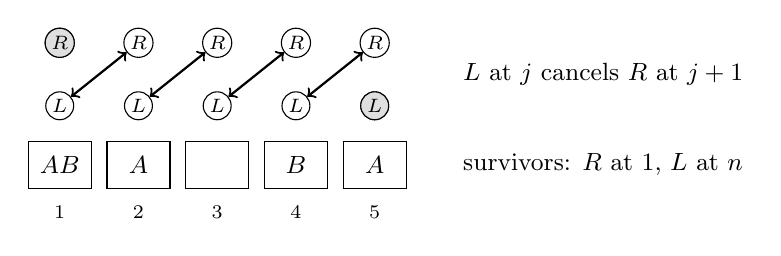
\begin{tikzpicture}[scale=1.0]
  \foreach \x/\lab in {1/{AB},2/{A},3/{},4/{B},5/{A}} {
    \draw (\x,0) rectangle (\x+0.8,0.6);
    \node at (\x+0.4,0.3) {\small $\lab$};
    \node at (\x+0.4,-0.3) {\scriptsize $\x$};
  }
  \foreach \x in {1,...,5} {
    \node[draw,circle,inner sep=1pt,font=\scriptsize] (L\x) at (\x+0.4,1.05) {$L$};
    \node[draw,circle,inner sep=1pt,font=\scriptsize] (R\x) at (\x+0.4,1.85) {$R$};
  }
  \foreach \x [evaluate=\x as \y using int(\x+1)] in {1,2,3,4} { \draw[<->,thick] (L\x) -- (R\y); }
  \node[draw,circle,inner sep=1pt,font=\scriptsize,fill=gray!25] at (1.4,1.85) {$R$};
  \node[draw,circle,inner sep=1pt,font=\scriptsize,fill=gray!25] at (5.4,1.05) {$L$};
  \node[anchor=west,font=\small] at (6.4,1.45) {$L$ at $j$ cancels $R$ at $j+1$};
  \node[anchor=west,font=\small] at (6.4,0.3) {survivors: $R$ at $1$, $L$ at $n$};
\end{tikzpicture}
\caption{The first count of $\mathcal T$ for a word of length $5$. Each flag $L$ at position $j$ cancels the flag
$R$ at position $j+1$; only $R$ at $1$ and $L$ at $n$ (shaded) survive. In the second count a flag is paired with the
other flag at its own position unless that position carries exactly one mark, as positions $2$, $4$ and $5$ do
here.}
\label{fig:telescope}
\end{figure}

\begin{proof}[Proof of Theorem~\ref{thm:main}]
By Lemmas~\ref{lem:bridge}, \ref{lem:cancel} and~\ref{lem:W},
\[
  (n+1)\,2^{n+1}(n-1)!\,|F_n|=(n+1)\,O_n=4\,n!\,(n+1)W_{n-1}=4\,n!\,2^n n!,
\]
so $|F_n|=2n\cdot n!/(n+1)$.
\end{proof}

\section{Remarks}\label{sec:remarks}

\emph{What is explicit.} Every step after Proposition~\ref{prop:GS} is an explicit sign-reversing involution or an
explicit insertion, and the bridge of Lemma~\ref{lem:bridge} is a term-by-term comparison of two finite counts. The
bijection behind Proposition~\ref{prop:GS} is obtained from a $2g$-to-$2g$ correspondence by Hall's theorem
\cite[\S2.4--2.5]{CFF}: a perfect matching can be found by exhaustive search, but no efficient or direct description is
known. So the proof is combinatorial throughout, but it does not give a direct bijection between the solutions and a
simpler set. A direct bijection, for instance between
the solutions with $u$ an $n$-cycle and a $1/n$ share of all solutions, is still open.

\emph{Why the count is not obvious.} The natural symmetries of the solution set do not explain the factor $n$. The
moves $(u,v)\mapsto(u,vu)$, $(u,v)\mapsto(uv,v)$ and $(u,v)\mapsto(cv,u^{-1})$ preserve the commutator, but their
orbits do not contain the solutions with $v$ an $n$-cycle in proportion $1/n$ (for $n=5$ the orbits have sizes $15$, $50$, $60$, $75$ and contain $5$, $25$, $10$, $0$ of them). This is
part of why we went through maps.

\emph{Verification.} Two programs that share no code check the identities (\ref{eq:three}). The first (Claude)
computes $|F_n|$ from all factorisations $c=\alpha\beta$ through (\ref{eq:zBi}), checks Proposition~\ref{prop:GS}
with $J=I$ against these factorisations for every composition, and computes $O_n$ and $W_{n-1}$ by brute force from
their definitions, for $n\le7$. The second (Codex) enumerates the solution pairs $(u,v)$ for $n\le9$, computes $O_n$
by cycle types for $n\le9$ and by direct enumeration for $n\le5$, evaluates $W_{n-1}$ over every marked word, and
checks the local sign maps and involutions exhaustively on small cases. The elementary identities used in Lemmas~\ref{lem:bridge} and~\ref{lem:W} are formalised in Lean 4.

\emph{Use of AI.} The cancellation argument of Sections~\ref{sec:cancel} and~\ref{sec:W} was found by OpenAI's Codex (model
GPT-6.1), working from a brief prepared in this project; Anthropic's Claude (Opus 5.5) prepared the earlier reductions, checked
every step of the argument and the computations independently, and drafted this note. The author directed the work and
is responsible for its content.

\begin{thebibliography}{9}
\bibitem{CFF} G.~Chapuy, V.~F\'eray and \'E.~Fusy, A simple model of trees for unicellular maps, \emph{J. Combin.
Theory Ser.~A} 120 (2013), 2064--2092; arXiv:1202.3252.
\bibitem{Boc} G.~Boccara, Nombre de repr\'esentations d'une permutation comme produit de deux cycles de
longueurs donn\'ees, \emph{Discrete Math.} 29 (1980), 105--134.
\bibitem{Chen} R.~X.~F.~Chen, A versatile combinatorial approach of studying products of long cycles in symmetric
groups, \emph{Adv. in Appl. Math.} 133 (2022), 102283; arXiv:1910.03571.
\bibitem{EC2} R.~P.~Stanley, \emph{Enumerative Combinatorics, Volume 2}, Cambridge University Press, 1999.
\bibitem{GS} A.~Goupil and G.~Schaeffer, Factoring $n$-cycles and counting maps of given genus, \emph{European J.
Combin.} 19 (1998), 819--834.
\bibitem{Bij} R.~P.~Stanley, Bijective proof problems, \url{https://math.mit.edu/~rstan/bij.pdf} (2009, revised
2015).
\end{thebibliography}
\end{document}
